\chapter{Aktuální projekty částečné dekarbonizace rafinérií}

V současné době se stále více pozornosti upíná k technologiím elektrolýzy vody, jelikož výroba zeleného vodíku představuje klíčový prvek pro částečnou dekarbonizaci nejen rafinérského průmyslu. Používání vodíku v rafinérských procesech je zodpovědné za přibližně $20\%$ celkových emisí vyprodukovaných z rafinerií, což představuje přibližně $230\ \mathrm{Mt_{CO_2}}$ za rok. \cite{IEAfuture} Částečné omezení a nahrazení výroby vodíku enviromentálně nešetrnými metodami, metodami \enquote{zelenými} je z ekonomických důvodů zatím v současnosti omezeno na demonstrační projekty, které budou představeny dále v této kapitole. V této souvislosti je vhodné si v krátkosti představit koncept vodíkového hospodářství, který s probíranou problematikou klimatické zátěže úzce souvisí.

\section{Vodíkové hospodářství}

Koncept vodíkové ekonomiky je založen na myšlence výroby vodíku z elektrické energie generované z obnovitelných zdrojů energie v období jejího nadbytku a opačným převodem v době nedostatku. \cite{Tkac2017} Další myšlenkou vodíkového hospodářství je optimalizace spojení jaderného reaktoru a \acs{SOEC} elektrolyzéru. Jaderné elektrárny produkují velkou tepelnou energii, který by se mohla využít pro elektrolyzér. \cite{Tkac2017}
\begin{figure}[h]
    \centering
    \begin{tikzpicture}
\node[inner sep=0pt] (obrazek) at (0,0)
    {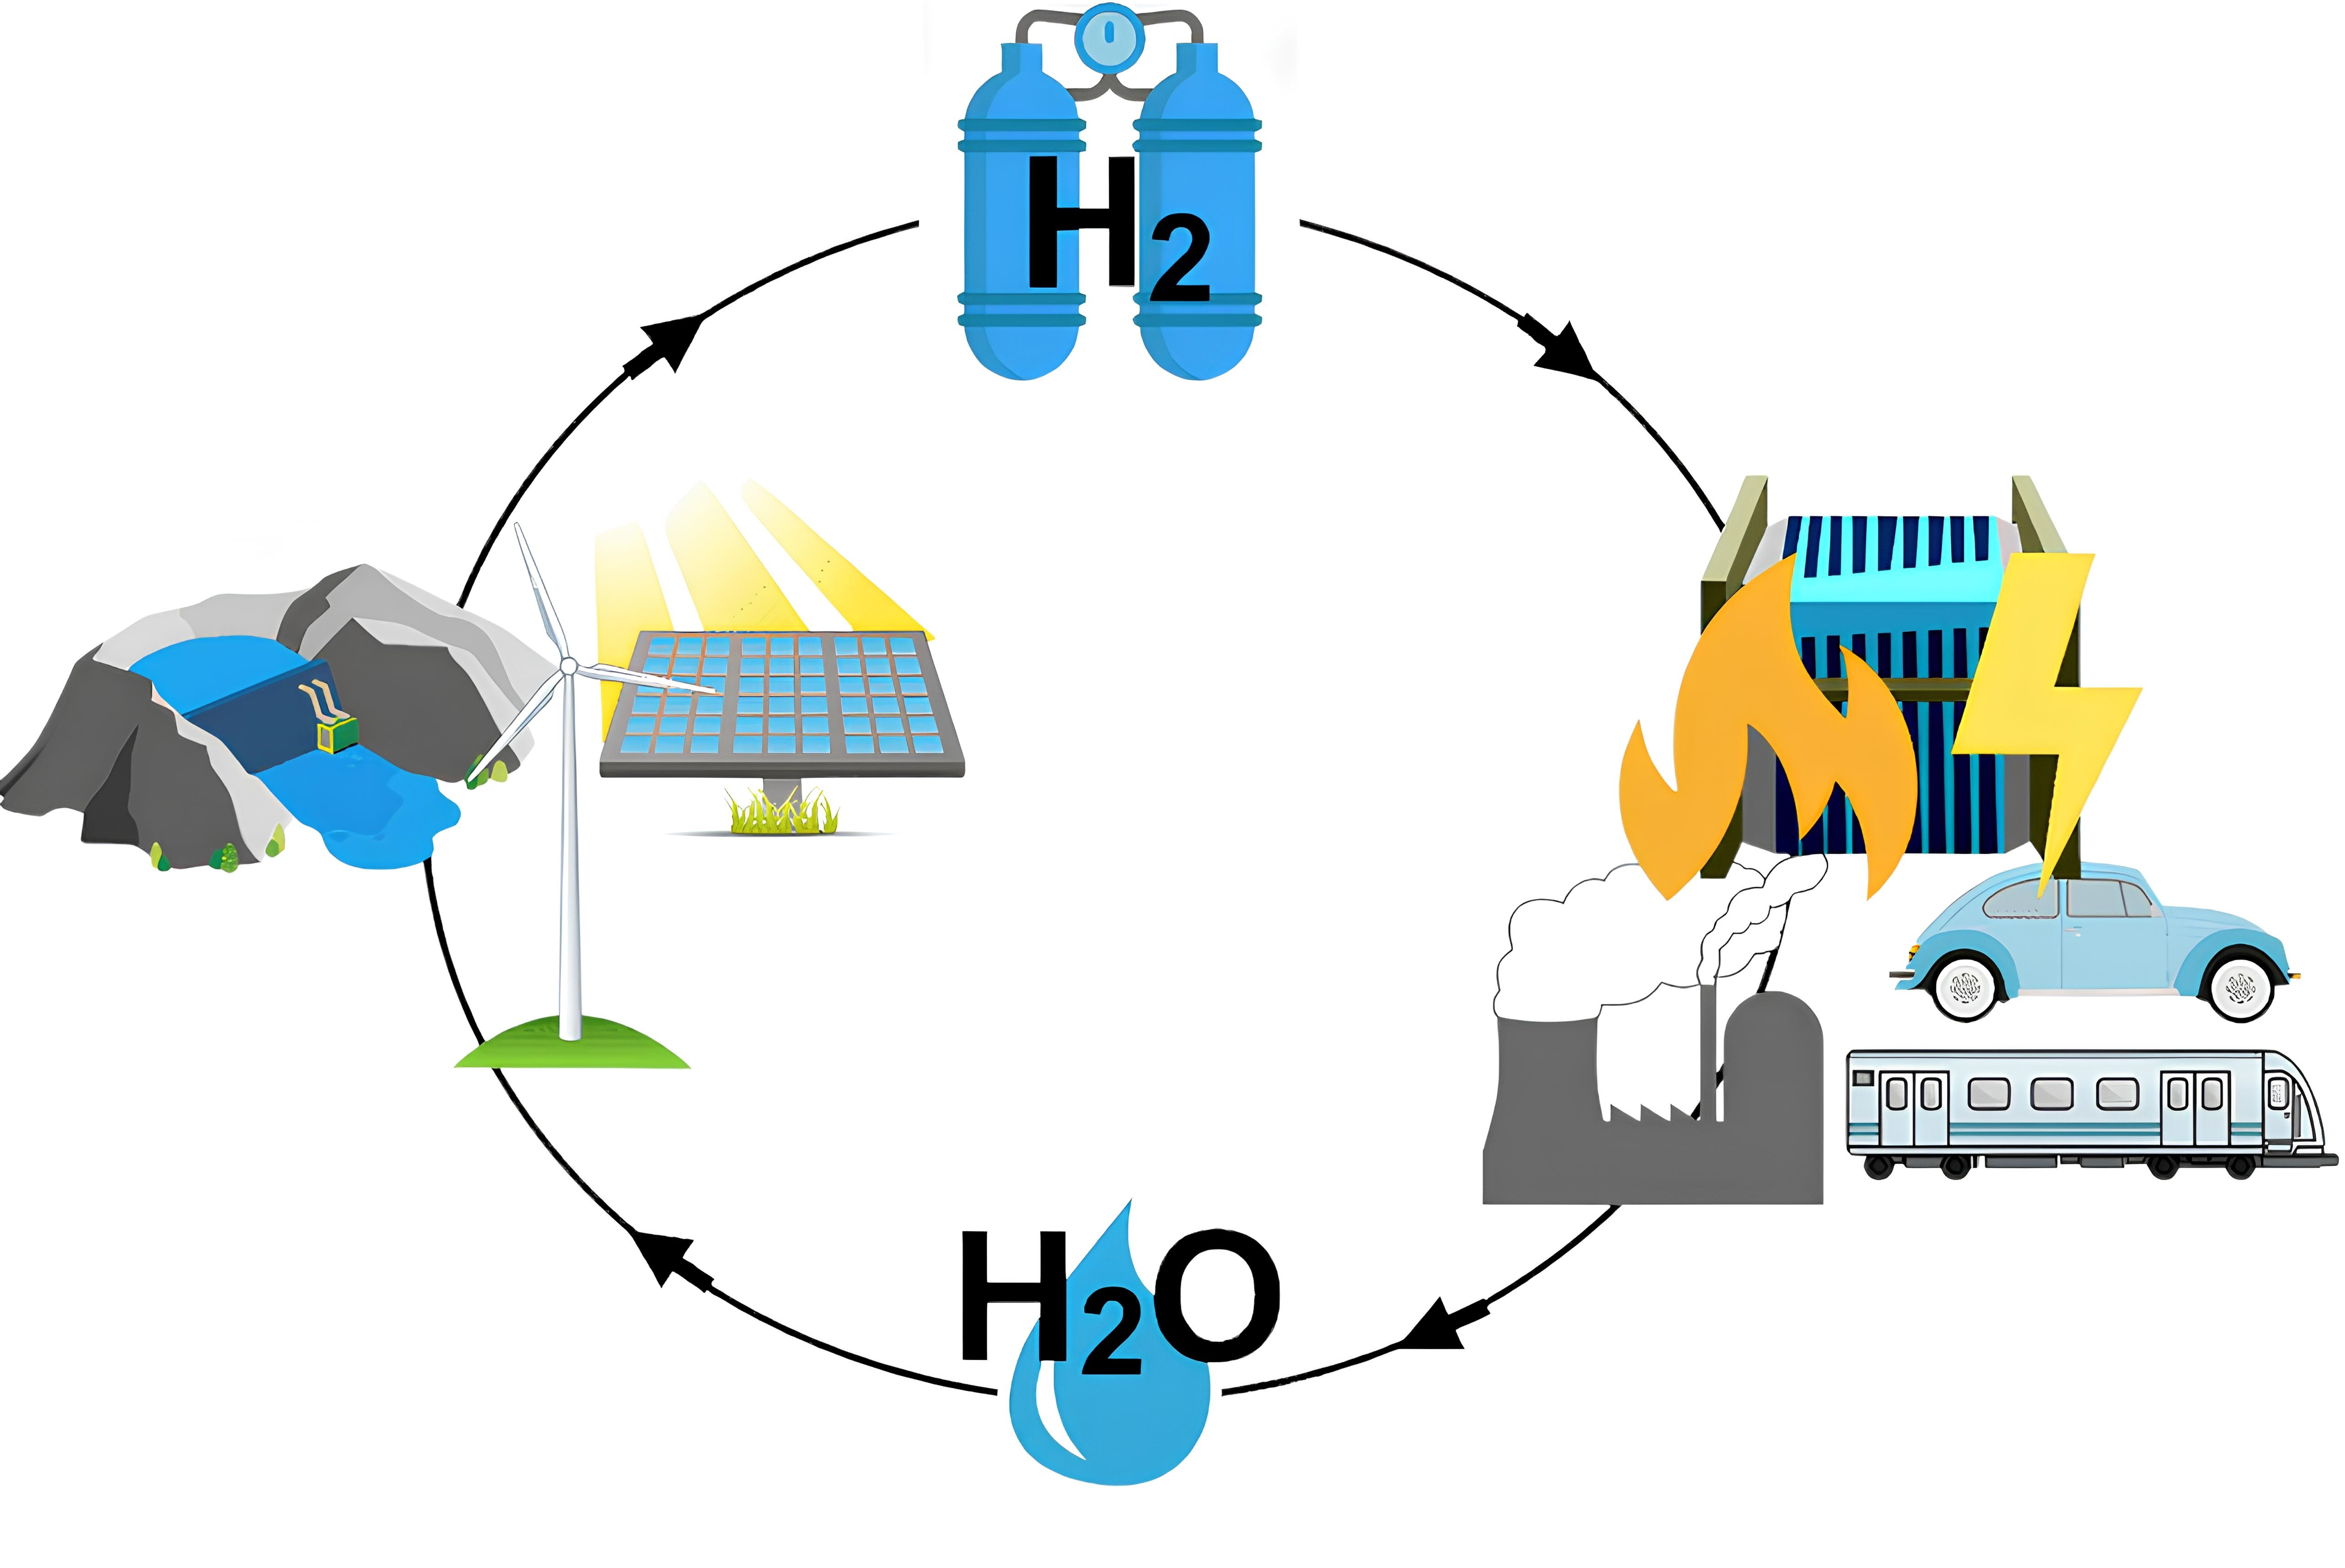
\includegraphics[width=0.8\textwidth]{figures/vodikove_hospodarstvi.jpg}};
\node[font=\small] at (-0.3,1.5) {nosič energie};
\node[font=\small] at (-0.35,-3.7) {voda};
\node[font=\small,align=center] at (3.85,-2.7) {Teplo, elektřina a\\spotřeba energie};
\node[font=\small,align=center] at (-4.8,-1.165) {Obnovitelné\\zdroje energie};
\end{tikzpicture}
    \caption[Princip vodíkového hospodářství]{Princip vodíkového hospodářství, převzato z \cite{Grahame2018}.} \label{fig:vodikove_hospodarstvi}
\end{figure}

Současným nedostatkem těchto myšlenek a jím podobným je však nedostatečná vodíková infrastruktura, tedy distribuční síť a velkokapacitní nízkoztrátové úložiště vodíku a to nejen v rafinériích. \cite{Tkac2017} Rozvinutí této infrastruktury je bez státní podpory ve formě dotací takřka nemožné a v souvislosti s tím si Česká republika, prostřednictvím Ministerstva průmyslu a obchodu, stanovila v publikaci \enquote{Vodíková strategie
České republiky} \cite{VodikovaStrategie} strategické cíle\footnote{Dle článku \cite{Votruba2024} není vodíková strategie v praxi dostatečně implementovaná a momentálně prochází aktualizací.}, které mají pomoci dosáhnout částečné klimatické neutrality do roku $2050$.

Dále je nutné zmínit, že se v nadcházejících letech bude i v Evropě prioritizovat dotační podpora právě projektů na rozvoj infrastruktury zeleného vodíku. Cílem je do roku $2030$ postavit elektrolyzéry o celkovém výkonu až $40\ \mathrm{GW}$ v rámci EU a podpořit výstavbu dalších $40\ \mathrm{GW}$ elektrolyzérů mimo území EU pro navýšení dovozu. \cite{Hytep} Kromě rozšíření výrobní kapacity vodíku se očekává, že technologický pokrok a zvýšení účinnosti samotných elektrolyzérů přispějí ke snížení ceny zeleného vodíku. 

\section{Projekty dekarbonizace rafinérského průmyslu}

Česká republika je vzhledem k absenci přístupu k moři odkázaná hlavně na obnovitelnou energii ze slunečního záření a větru. Projekt firmy \textit{Orlen Unipetrol RPA s.r.o.} v Litvínově - Záluží představený v následující podkapitole realizuje využití elektrické energie získané pravě fotovoltaickými panely na výrobu zeleného vodíku v elektrolyzéru. Ostatní evropské země mají v ohledu obnovitelné energie více možností. Pozornost bude věnována především na projekty v nizozemském Rotterdamu, kde leží největší námořní přístav v Evropě.

\subsection{Orlen Unipetrol - Litvínov, Česká republika}

Tuzemské rafinérie \textit{Orlen Unipetrol} v Litvínově - Záluží, která je od roku 2004 ve vlastnictví polské petrochemické společnosti \textit{PKN Orlen} \cite{unipetrol_historie}, plánuje na přelomu let 2024 a 2025 začít stavět novou fotovoltaickou elektrárnu o instalovaném výkonu až $60\ \mathrm{MW}$. Elektrická energie generovaná vlastními fotovoltaickými systémy však nebude dostatečná pro produkci zeleného vodíku. Z tohoto důvodu bude \textit{Orlen Unipetrol} nakupovat zelenou energii také od externích dodavatelů, aby zajistil provoz elektrolyzéru i během nočních hodin. \cite{Votruba2024}
\begin{figure}[h]
    \centering
    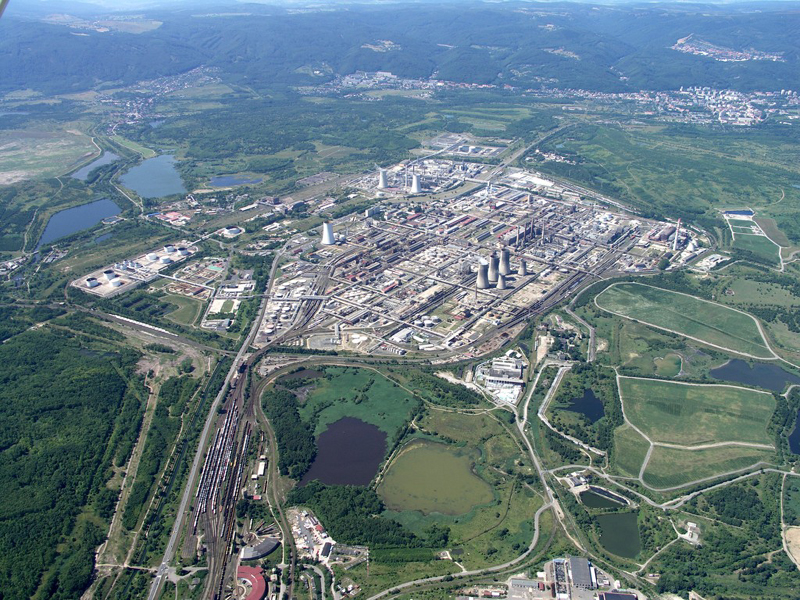
\includegraphics[width=.6\textwidth]{figures/letecky_snimek.png}
    \caption[Letecký snímek rafinérie \textit{Orlen Unipetrol} s přilehlým areálem]{Letecký snímek rafinérie \textit{Orlen Unipetrol} s přilehlým areálem \cite{hydrokrak_litvinov}.} \label{fig:letecky_snimek}
\end{figure}

Současně s tím byl v minulých letech oznámen projekt stavby elektrolyzéru, který by na svůj provoz využíval elektrickou energii ze zmíněné solární elektrárny. Elektrolyzér, jehož instalovaný výkon dosahuje až $26\ \mathrm{MW}$, by měl po předpokládaném dokončení stavby v roce 2028 produkovat až $4,5\ \mathrm{kt}$ zeleného vodíku ročně. \cite{Soucek2023} Předpokládaná investice do celého komplexu v litvínovské rafinérii je ve výši až 3 miliard Kč. \cite{unipetrol_zprava,Soucek2023} Celý areál má být postaven v areálu zaniklé vesnice Růžodol v těsné blízkosti tamní rafinérie, znázorněný na Obr. \ref{fig:letecky_snimek}. \cite{Votruba2024}

Pro dekarbonizaci rafinérských a petrochemických aktivit firmy \textit{Orlen Unipetrol} je potřeba dle dat samotné firmy dosáhnout do roku 2030 produkce přibližně $43,8\ \mathrm{kt}$ obnovitelného vodíku ročně. \cite{unipetrol_zprava}

\subsection{Zeeland Refinery - Nieuwdorp, Nizozemsko}

Rafinérie \enquote{Zeeland}, která je ve vlastnictví firem \textit{Total Energies} a \textit{Lukoil}, leží v pobřežní průmyslové části vesnice Nieuwdorp, kde ročně vyprodukuje až $11,5$ milionů tun produktů ročně. Mezi tyto produkty patří samozřejmě paliva, topné oleje, ale i rozpouštědla a suroviny pro výrobu plastů. \cite{Zeeland}

Projekt této firmy na částečnou dekarbonizaci své rafinerie byl představen v roce 2021 a jeho cílem projektu je do roku 2026 postavit elektrolyzér o výkonu $150\ \mathrm{MW}$ s cílem produkovat až $21\ \mathrm{kT}$ vodíku ročně. \cite{deLaat2022} Společně s již vystavenou solární elektrárnou (viz. Obr. \ref{fig:Zeeland_solarnipark}) o instalovaném výkonu přibližně $11\ \mathrm{MW}$, která již nyní pokrývá spotřebu celé rafinérie z $22\%$, má projekt kvůli výborné volbě lokality potenciál na dekarbonizaci rafinérie. \cite{Zeeland} Projekt je aktuálně ve fázi předběžného technického návrhu a má být dokončen v roce 2026. \cite{deLaat2022}
\begin{figure}[h]
    \centering
    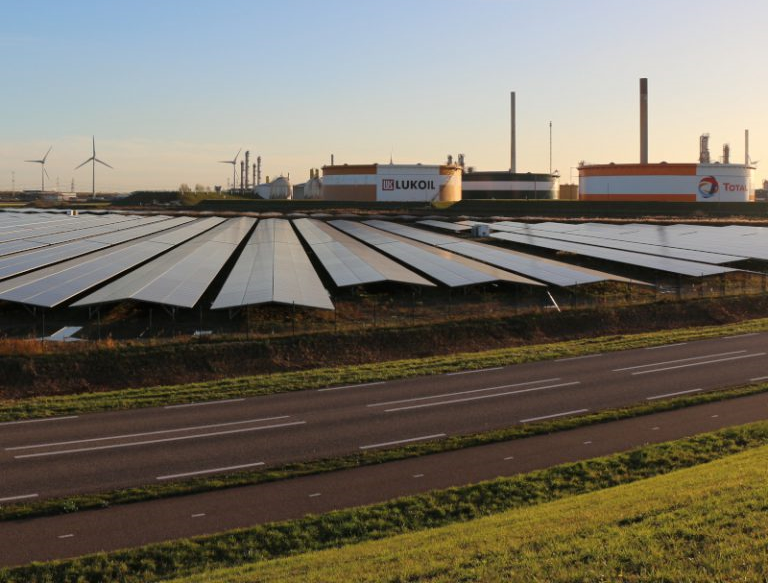
\includegraphics[width=.7\textwidth]{figures/Zeeland_solarnipark.png}
    \caption[Solární park rafinérie \enquote{Zeeland}]{Solární park rafinérie \enquote{Zeeland} \cite{Zeeland}.} \label{fig:Zeeland_solarnipark}
\end{figure}

Kromě již zmíněného projektu výroby obnovitelného vodíku má rafinerie \enquote{Zeeland} projekt i na výrobu nízkouhlíkového, modrého, vodíku. Cílem tohoto projektu je snížení uhlíkových emisí produkovaných při výrobě vodíku ze zemního plynu pomocí technologií \acs{CCS} až na polovinu oproti aktuálnímu stavu. Produkovaný oxid uhličitý má být v novém zařízení zachycován a zkapalňován. Zkapalněný oxid uhličitý se pak za pomoci lodní dopravy umístí do tzv. plynových polí v Severním moři, kde je trvale uchováván. Projekt \enquote{Azur}, jak je nazýván podle barvy produkovaného vodíku, má být dokončen ve třetím čtvrtletí roku 2026. \cite{Zeeland}

\subsection{Shell Energy and Chemicals Park - Rotterdam, Nizozemsko}

Dominantním subjektem mezi všemi zamýšlenými projekty v nizozemském přístavu je energetický park a rafinerie firmy \textit{Shell}. Denně zde zpracují na $65\ 000\ \mathrm{m^3}$ ropy, ze které produkují převážně plynový olej a naftu. V přilehlých chemických závodech jsou produkovány rozpouštědla různých druhů. \cite{Shell}

V areálu o ploše $5\ 5000\ 00\ \mathrm{m^2}$ by měl v roce 2025 uveden do provozu jeden z největších závodů na výrobu zeleného vodíku v Evropě. Elektrolyzér o výkonu $200\ \mathrm{MW}$ má produkovat až $80\ \mathrm{t}$ vodíku denně nejen pro potřeby rafinérie. Výkonný elektrolyzér je samozřejmě zásobován elektrickou energií z mimopobřežních větrných elektráren v Severním moři, které z $80\%$ vlastní také \textit{Shell}. \cite{ShellGlobal2022}
\begin{figure}[h]
    \centering
    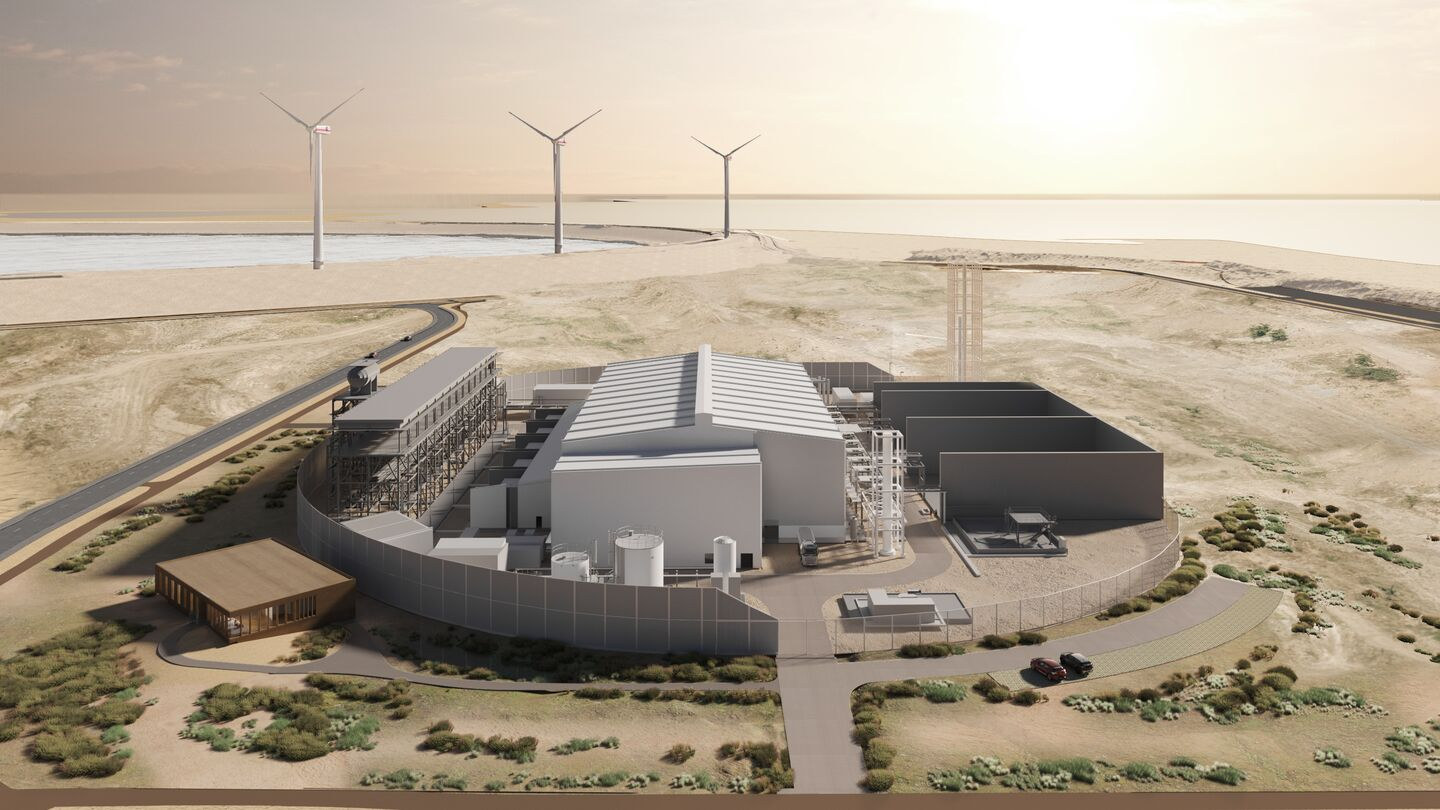
\includegraphics[width=.75\textwidth]{figures/shell_rotterdam.jpg}
    \caption[Vizualizace projektu \enquote{Holland Hydrogen 1} firmy \textit{Shell}]{Vizualizace projektu \enquote{Holland Hydrogen 1} firmy \textit{Shell} \cite{shell_rotterdam}.} \label{fig:shell_rotterdam}
\end{figure}

Nahrazení produkce šedého vodíku enviromentálně šetrnějším vodíkem zeleným může ročně zamezit vypuštění až $200\ 000\ \mathrm{t}$ oxidu uhličitého. \cite{deLaat2022}

\subsection{British Petroleum - Rotterdam, Nizozemsko}

Dalším významným subjektem operujícím v největším námořním přístavu v Evropě je nizozemská divize firmy \textit{British Petroleum}. Ta společně s \textit{Hydrogen Chemistry Company} představila v roce 2019 dosud největší projekt pod názvem \enquote{H2-Fifty}. H2-Fifty je významný environmentálně šetrný projekt zaměřený na produkci zeleného vodíku, který má za cíl podpořit vodíkovou strategii celého rotterdamského přístavu. Elektrolyzér o výkonu až $250\ \mathrm{MW}$ s roční produkcí $40\ \mathrm{kt}$ částečně omezí uhlíkovou stopu tamní rafinerie, ale i ostatních průmyslových odvětví v rotterdamském přístavu a širším regionu Beneluxu. \cite{bpnederland2024} V rafinierii \textit{British Petroleum} se vodík využívá primárně na hydrogenační rafinaci ropných produktů. \cite{deLaat2022}
\newpage
\begin{figure}[h]
    \centering
    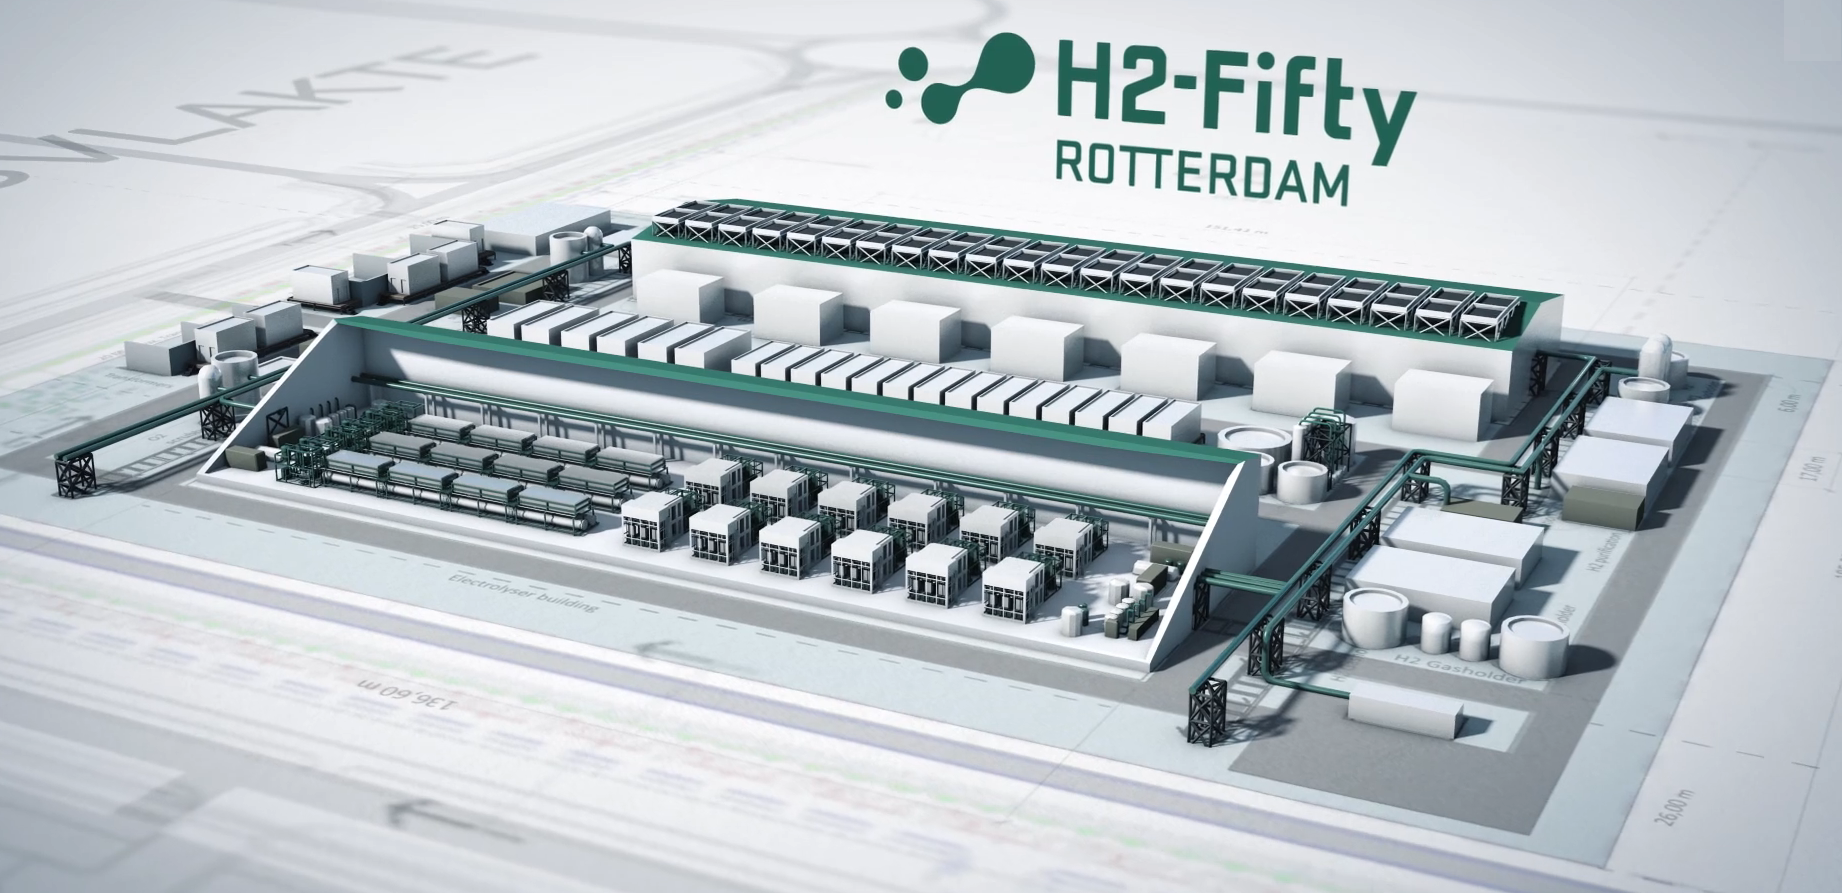
\includegraphics[width=.8\textwidth]{figures/h2fifty.png}
    \caption[Vizualizace projektu \enquote{H2-Fifty} firmy \textit{bp \& HyCC}]{Vizualizace projektu \enquote{H2-Fifty} firmy \textit{bp \& HyCC} \cite{HyCC2024}.} \label{fig:h2fifty}
\end{figure}

Protože je zelený vodík ze své definice vyráběný z elektrické energie pocházející z obnovitelných zdrojů energie, může tento projekt snížit vypouštění oxidu uhličitého do ovzduší z rafinérie \textit{British Petroleum} až o $300\ 000\ \mathrm{t}$ ročně. Projekt je aktuálně ve fázi implementace a náklady na výstavbu se pohybují v intervalu $225 \div 300$ milionů eur. \cite{deLaat2022} 

\subsection{Neste - Porvoo, Finsko}

Na jihu Finska v přístavním městě Porvoo provozuje tamní společnost \textit{Neste} rafinérii, která má výrobní kapacitu přibližně $1\ 200\ 000\ \mathrm{t}$ ropných produktů ročně. Cílem této společnosti je společně s jejími partnery dosáhnout uhlíkové neutrality do roku 2040 a stát se jednou z nejudržitelnějších rafinérií v Evropě. \cite{Neste2024}

Rafinérie, jež využívá i lokální fotovoltaické elektrárny pro dodávku elektrické energie \cite{Neste2023}, produkuje ročně přibližně $2\ 800\ 000\ \mathrm{t}$ oxidu uhličitého. Rafinérii čeká částečné zmírnění nepříznivého enviromentálního dopadu v roce 2026, kdy má být uveden do provozu elektrolyzér o výkonu $120\ \mathrm{MW}$, který bude rafinérii zásobovat zeleným vodíkem. \cite{Neste2023a} Projekt, který vznikl teprve v roce 2023, má v plánu implementovat 6 jednotek elektrolyzéru \enquote{scalum} německé firmy \textit{thyssenkrupp nucera}. \cite{thyssenkruppnucera2023} Každá z nich je schopná produkovat až $4000\ \mathrm{Nm^3}$ vodíku za hodinu. Jednotky jsou kompaktní, dají se řadit za sebe až do výkonu $1\ \mathrm{GW}$. \cite{thyssenkruppnucera2023a}
\begin{figure}[h]
    \centering
    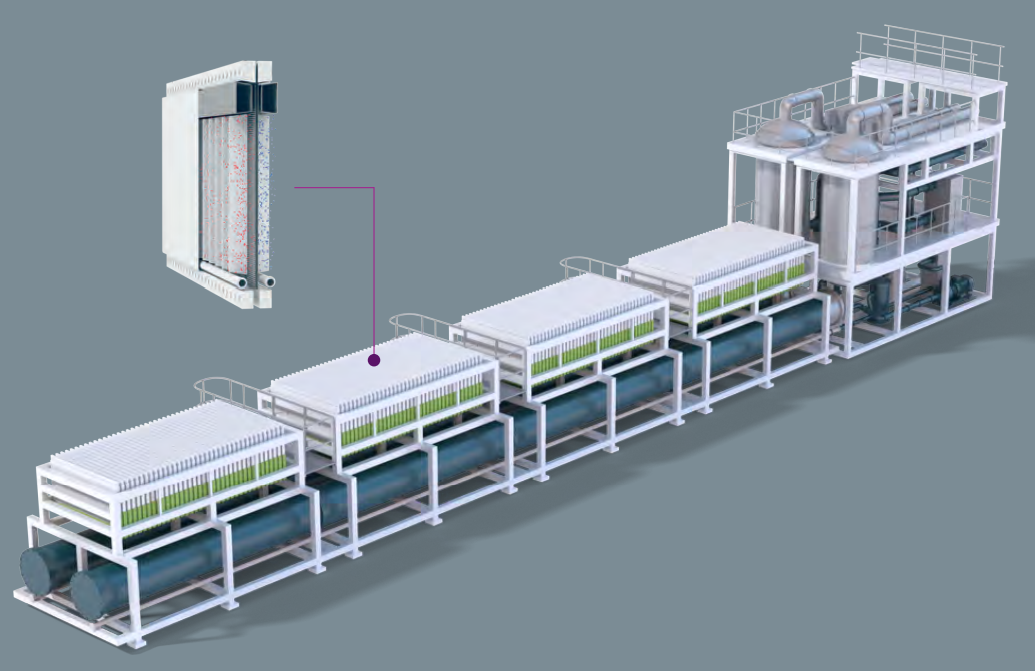
\includegraphics[width=.7\textwidth]{figures/scalum.png}
    \caption[Elektrolyzér \enquote{scalum} firmy \textit{thyssenkrupp nucera}]{Elektrolyzér \enquote{scalum} firmy \textit{thyssenkrupp nucera} \cite{thyssenkruppnucera2023a}.} \label{fig:scalum}
\end{figure}